% CVPR 2022 Paper Template
% based on the CVPR template provided by Ming-Ming Cheng (https://github.com/MCG-NKU/CVPR_Template)
% modified and extended by Stefan Roth (stefan.roth@NOSPAMtu-darmstadt.de)

\documentclass[10pt,twocolumn,letterpaper]{article}

%%%%%%%%% PAPER TYPE  - PLEASE UPDATE FOR FINAL VERSION
%\usepackage[review]{cvpr}      % To produce the REVIEW version
\usepackage{cvpr}              % To produce the CAMERA-READY version
%\usepackage[pagenumbers]{cvpr} % To force page numbers, e.g. for an arXiv version

% Include other packages here, before hyperref.
\usepackage{graphicx}
\usepackage{amsmath}
\usepackage{amssymb}
\usepackage{booktabs}
\usepackage{float}


% It is strongly recommended to use hyperref, especially for the review version.
% hyperref with option pagebackref eases the reviewers' job.
% Please disable hyperref *only* if you encounter grave issues, e.g. with the
% file validation for the camera-ready version.
%
% If you comment hyperref and then uncomment it, you should delete
% ReviewTempalte.aux before re-running LaTeX.
% (Or just hit 'q' on the first LaTeX run, let it finish, and you
%  should be clear).
\usepackage[pagebackref,breaklinks,colorlinks]{hyperref}


% Support for easy cross-referencing
\usepackage[capitalize]{cleveref}
\crefname{section}{Sec.}{Secs.}
\Crefname{section}{Section}{Sections}
\Crefname{table}{Table}{Tables}
\crefname{table}{Tab.}{Tabs.}


%%%%%%%%% PAPER ID  - PLEASE UPDATE
\def\cvprPaperID{****} % *** Enter the CVPR Paper ID here
\def\confName{CVPR}
\def\confYear{2023}

\begin{document}

%%%%%%%%% TITLE - PLEASE UPDATE
\title{Unmasking Sarcasm - Enhancing Sentiment Analysis in E-Commerce Reviews and Questions
}

\author{Hugo Bouy\\
Illinois Tech\\
{\tt\small hbouy@hawk.iit.edu}
% For a paper whose authors are all at the same institution,
% omit the following lines up until the closing ``}''.
% Additional authors and addresses can be added with ``\and'',
% just like the second author.
% To save space, use either the email address or home page, not both
\and
Rémi Kalbe\\
Illinois Tech\\
{\tt\small rkalbe@hawk.iit.edu}
\and
Mathias Roumane\\
Illinois Tech\\
{\tt\small mroumane@hawk.iit.edu}
}
\maketitle

%%%%%%%%% ABSTRACT
% \begin{abstract}
%    The ABSTRACT is to be in fully justified italicized text, at the top of the left-hand column, below the author and affiliation information.
%    Use the word ``Abstract'' as the title, in 12-point Times, boldface type, centered relative to the column, initially capitalized.
%    The abstract is to be in 10-point, single-spaced type.
%    Leave two blank lines after the Abstract, then begin the main text.
%    Look at previous CVPR abstracts to get a feel for style and length.
% \end{abstract}

%%%%%%%%% BODY TEXT
\section{Problem description}
\label{sec:intro}
In an increasingly e-commerce driven world, the analysis of review, comments and questions written by consumers online has become a field of interests. Understanding opinions and emotions expressed in product feedback/related questions is essential to enhance the user’s experience. One aspect that might be overlooked in this area is sarcastic and humor detection that can lead to a misinterpretation of these texts.

Humor remains a complex human phenomenon that is far from having a clear definition. While humor and sarcastic mechanisms are integral to human interaction, its subjective nature makes it a challenging target for computational analysis. Recent work has been able to open up this area using deep learning and natural language processing advances. With this project, we will attempt to improve e-commerce review processing using deep learning models for humor disambiguation.


%-------------------------------------------------------------------------
\section{Datasets}
\subsection{Combined dataset for sarcasm detection}

To train this model, we used a collection of dataset of sentences. The main datasets used in the scope of this project is given below.
\begin{itemize}
    \item {\bfseries Headlines dataset}: Contains a list of 28,619 headlines collected from two news website. On one hand, TheOnions aims at producing sarcastic versions of real news events. On the other hand, real and non sarcastic news headloines are collected form HuffPost. This dataset has the advantage of having no spelling mistakes and informal usage since it is written by dedicated professionals in a formal manner.
    \item {\bfseries MUStARD++ dataset}: Mustard++ is a multimodal sarcasm dataset that has been anotated whith 9 emotions. It was compiled form popular TV shows such as Friends, The Golden Girls or The Big Bang Theory. We will be using this dataset mostly to detect sarcasm but if we have time we may use the annotation to classify the emotion associated with the sarcastic sentence considered.
    \item {\bfseries Sarcasm Corpus V2 dataset}: This dataset contains both sarcastic and non-sarcastic utterances. They are additionally classified in three different types: generic (6,520 samples), hyperbole (1.164 samples) and rhetorical (1,702 samples).
    \item {\bfseries Sarcasm Amazon reviews dataset}: Contains a large number of both regular and ironic Amazon reviews. Each review is also associated with informations about the product for which the review was written, the number of stars assigned by the author, etc. This dataset will be the most usefull in the secind part of our project when we link the sarcastic review with the information regarding the product.
\end{itemize}
As an initial data processing step, we first concatenated those datasets together in order to use them to implement an initial sarcasm detection model. The final combined dataset then has the full sentence or review and a sarcastic indicator (0 or 1). The final combined dataset contains 40,461 samples from different sources and types. We then have a quite complex dataset with sentences of very variable length as displayed in figure \ref*{sentence_fig}.
\begin{figure}[]
    \centering
    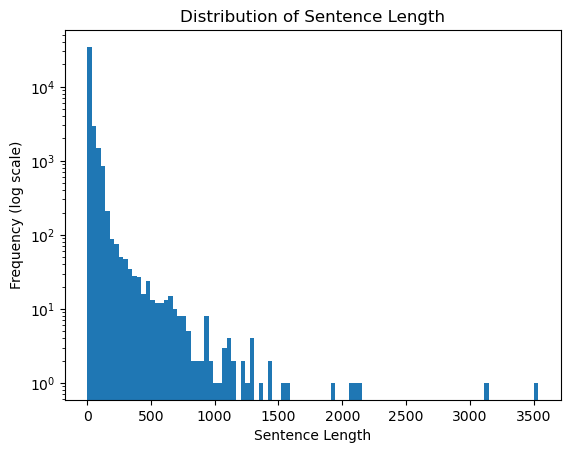
\includegraphics[width=0.8\linewidth]{Figure_sentence_length.png}
    \caption{Frequency of sentence length in the final combined dataset}
    \label[type]{sentence_fig}
\end{figure}

\subsection{Amazon reviews dataset}


%-------------------------------------------------------------------------
\section{Results}
\subsection{Simple Sarcasm detection model}
As a starting point for this project, we first aimed at creating a simple model capable of detecting if a sentence contains some form of sarcasm. At this stage, the model only takes into account the sentence and no additional factors. We were able to later on add additional relevant factors in detecting sarcastic or humorous patterns such as information on the product considered. 

Our best results were obtained using the BERT pre-trained model. BERT or "Bidirectional Encoder Representations from Transformers", is a widely used pretrained natural language processing model developed in 2018. This model is built on a transformer architecture which enables efficient handling of sequential data. Additionally, it has already been trained on a massive amout of text data making an ideal choice for any specific NLP task after fine-tuning. Additionally, BERT uses a bidirectional approach making it possible to consider the entire context of a word in any given sentence making it better at capturing the nuance and complexity of laguage.
Those few characteristics makes this state-of-the-art deep neural network ideal to capture the intricacies of a complex human behaviour such as sarcasm.


\subsection{Sarcasm detection with additional factors}

\subsection{Comparison with Chat-GPT}
In order to enhance the depth of our analysis, we conducted a comparative evaluation between our sarcasm detection model and Chat-GPT, primarily focusing on the GPT-3.5-turbo variant developed by OpenAI.
The objective of this comparison was to assess the efficacy of our model in comparison to a widely recognized general-purpose language model.

\subsubsection{Methodology}
Our approach involved querying Chat-GPT with a set of sentences from our dataset, asking it to determine if each was sarcastic.
The queries were formulated in a simple way, while we recognize that the design of the prompt was not extensively optimized and may need more modification to improve accuracy.
This observation suggests the possibility of making enhancements in further experimental endeavors.

\subsubsection{Observations}
The preliminary results of Chat-GPT on our sarcasm detection test were unsatisfactory, exhibiting an accuracy rate of merely 59.75\%.
The actual application of Chat-GPT was hindered by the time-consuming nature of its interaction, mostly caused by the response latency and rate limiting of the API. This limitation had a notable impact on the usability of Chat-GPT in many circumstances.
Furthermore, the responses generated by Chat-GPT occasionally deviated from the intended aim, most likely related to its broad training and reliance on the provided prompts.

Moreover, the financial aspect associated with the utilization of GPT-3.5-turbo proved to be significant, especially considering its rather limited precision as observed in our conducted evaluations.
Taking into account these factors, including the processing requirements and concerns regarding response time, raises doubts about the viability of utilizing this approach for sarcasm detection in e-commerce environments on a big scale or in real-time scenarios.
Subsequent examinations may be conducted to assess the potentialities of GPT-4; nevertheless, the substantial cost associated with its utilization constitutes a pivotal aspect requiring careful deliberation.

%-------------------------------------------------------------------------

\section{What is left to be done}

Our project focus on how sentiment analysis tools dedicated to sarcasm and humor disambiguation can be used to enhance E-commerce review and Q\&A processing.
It can be divided in 5 main milestones:

\begin{enumerate}
    \item First, we implement a basic model able to detect humor/sarcasm in small text reviews. This model would only be capable of saying whether or not a given phrase/text contains humor or sarcasm patterns. To build the model, we compare different approaches published in the scientific literature.
    
    \item Second, we improve the model to take into account several factors such as the type of product considered, its description, price, etc. (as sarcasm may be related to one aspect of the product). Feeding the model with the context can also help identify if some type of products are more prone to trigger humorous or sarcastic comments.
    
    \item Third, we compare our model to a LLM such as ChatGPT to assess if our dedicated humor/sarcasm classification model performs significantly better than a state of the art LLM using an appropriate prompt. We analyze the cost of both solutions.
    
    \item Fourth, we improve our model to properly classify a product review considering its sarcastic/humorous sense into meaningful categories such as "consumer thinks the product is overpriced", "consumer thinks the product is good quality", etc. For instance, humor regarding the price of a product may indicate the product is overpriced compared to the customer’s expectations.
    
    \item If time allows it, we will use our sarcastic model detection to generate relevent automatic answer that take into account the humorous tone of the comment/question.
\end{enumerate}

%%%%%%%%% REFERENCES

\nocite{*}
{\small
\bibliographystyle{ieee_fullname}
\bibliography{egbib}
}

\end{document}
